\section{Experimental Evaluation}
\label{sec:experiment}

In this section, we conduct a practical evaluation through experimentation in 
which we instantiate the semantic models (Figure~\ref{fig:wicusrels}) for three real 
scientific workflow applications. We study and document the Montage~\cite{Montage},
Epigenomics~\cite{genome}, and SoyKB~\cite{soybean, Joshi01012014} workflows 
and their execution environments, which include the application software components 
and the workflow management system.

The goal of this experiment is to reproduce original workflow executions in two different 
Cloud infrastructures, FutureGrid~\cite{futuregrid} and Amazon EC2~\cite{aws}, and a
local execution environment by using Vagrant. 
FutureGrid is an academic Cloud test-bed facility that includes a number of computational 
resources at distributed locations. Amazon Web Services EC2 is a public infrastructure 
provider and the \emph{de facto} standard for IaaS Cloud platforms. 


\subsection{Scientific Workflows}

\paragraph{\textbf{Montage}}
The Montage workflow~\cite{Montage} was created by the NASA Infrared Processing 
and Analysis Center (IPAC) as an open source toolkit that can be used to generate 
custom mosaics of astronomical images in the Flexible Image Transport System (FITS) 
format. In a Montage workflow, the geometry of the output mosaic is calculated from the 
input images. The inputs are then re-projected to have the same spatial scale and rotation, 
the background emissions in the images are corrected to have a uniform level, and the 
re-projected, corrected images are co-added to form the output mosaic. 
Figure~\ref{fig:workflow-montage} illustrates a small (20 node) Montage workflow. The 
size of the workflow depends on the number of images required to construct the desired 
mosaic.

\begin{figure}[!htt]
	\centering
	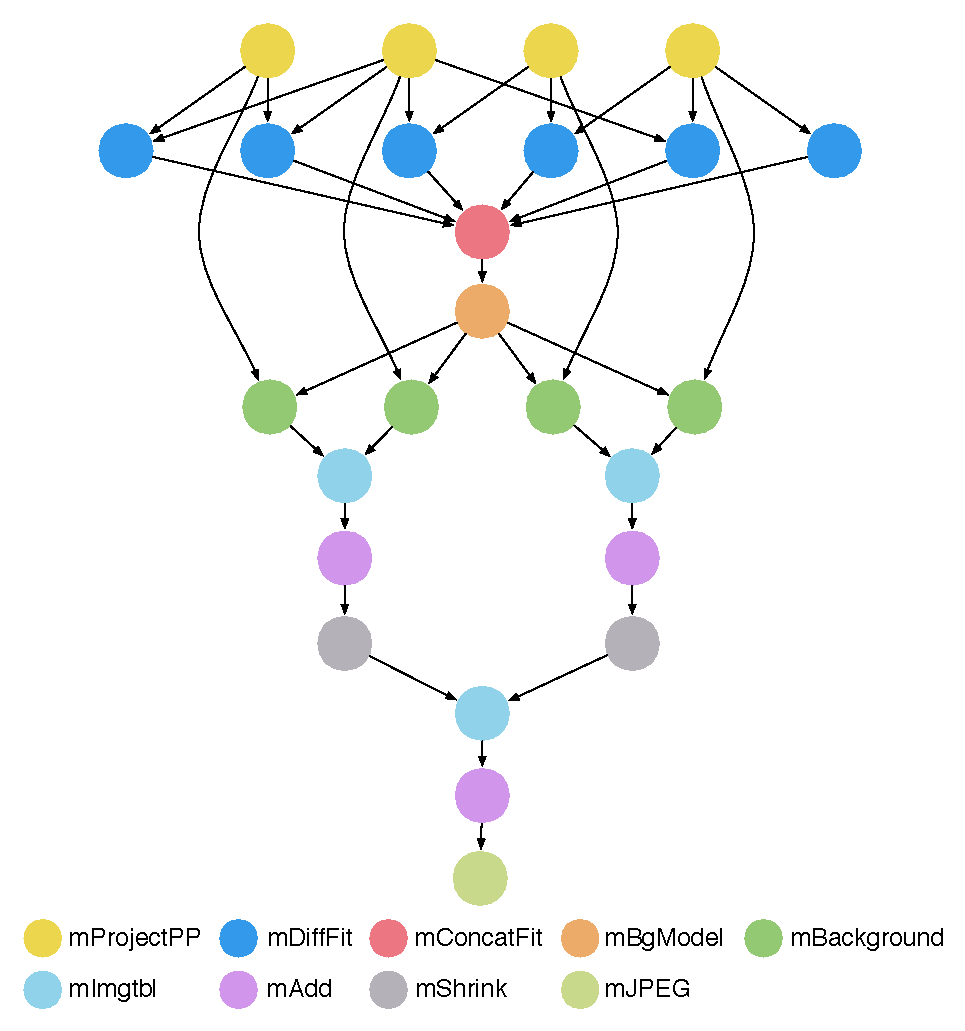
\includegraphics[width=0.9\linewidth]{figures/workflow-montage}
	\caption{A small (20 node) Montage workflow.}
	\label{fig:workflow-montage}
\end{figure}


\paragraph{\textbf{Epigenomics}}
The USC Epigenome Center~\cite{genome} is currently involved in mapping the epigenetic 
state of human cells on a genome-wide scale. The Epigenomics workflow 
(Figure~\ref{fig:workflow-genome}) processes multiple sets of genome sequences in
parallel. These sequences are split into subsets, the subsets are filtered to remove
contaminants, reformatted, then mapped to a reference genome. The mapped sequences are
finally merged and indexed for later analysis. In this work, the Epigenome workflow was 
used to align genome sequence reads to a reference genome for human chromosome 
21. The size of the workflow depends on the chunking factor used on the input data, 
which determines the number of sequence reads in each chunk.

\begin{figure}[!htb]
	\centering
	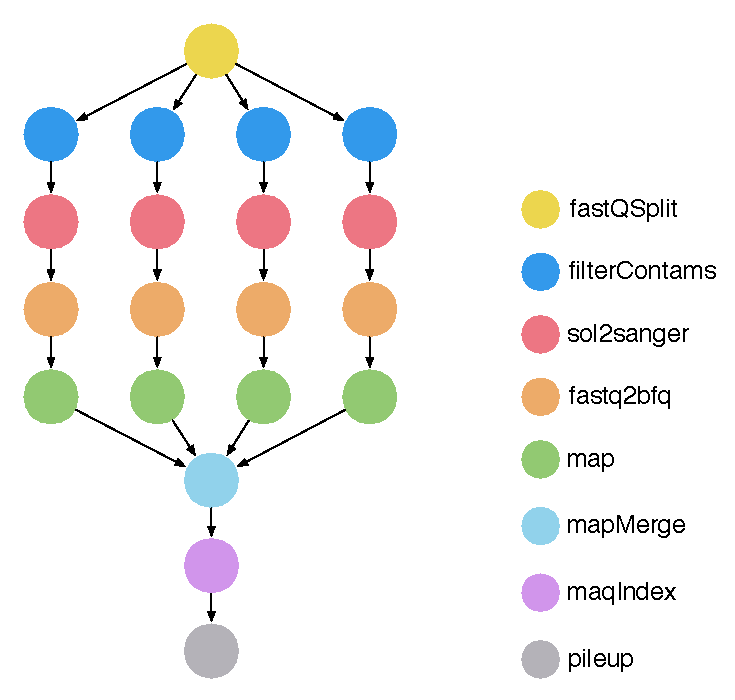
\includegraphics[width=0.75\linewidth]{figures/workflow-genome}
	\caption{Epigenomics workflow.}
	\label{fig:workflow-genome}
\end{figure}

\paragraph{\textbf{SoyKB}}
The SoyKB workflow~\cite{soybean, Joshi01012014} is a genomics pipeline 
that re-sequences soybean germplasm lines selected for desirable traits such 
as oil, protein, soybean cyst nematode resistance, stress resistance, and root 
system architecture. The workflow (Figure~\ref{fig:workflow-soykb}) 
implements a SNP and injection/deletion (indel) identification and analysis 
pipeline using the GATK haplotype caller~\cite{gatk} and a soybean reference 
genome. The workflow analyzes samples in parallel to align them to the reference 
genome, to de-duplicate the data, to identify indels and SNPs, and to merge and 
filter the results. The results are then used for genome-wide association studies 
(GWAS) and genotype to phenotype analysis. The workflow instance used in this 
paper is based on a sample dataset that requires less memory than a full-scale 
production workflow, however it requires the same software components.

\begin{figure}[!htb]
	\centering
	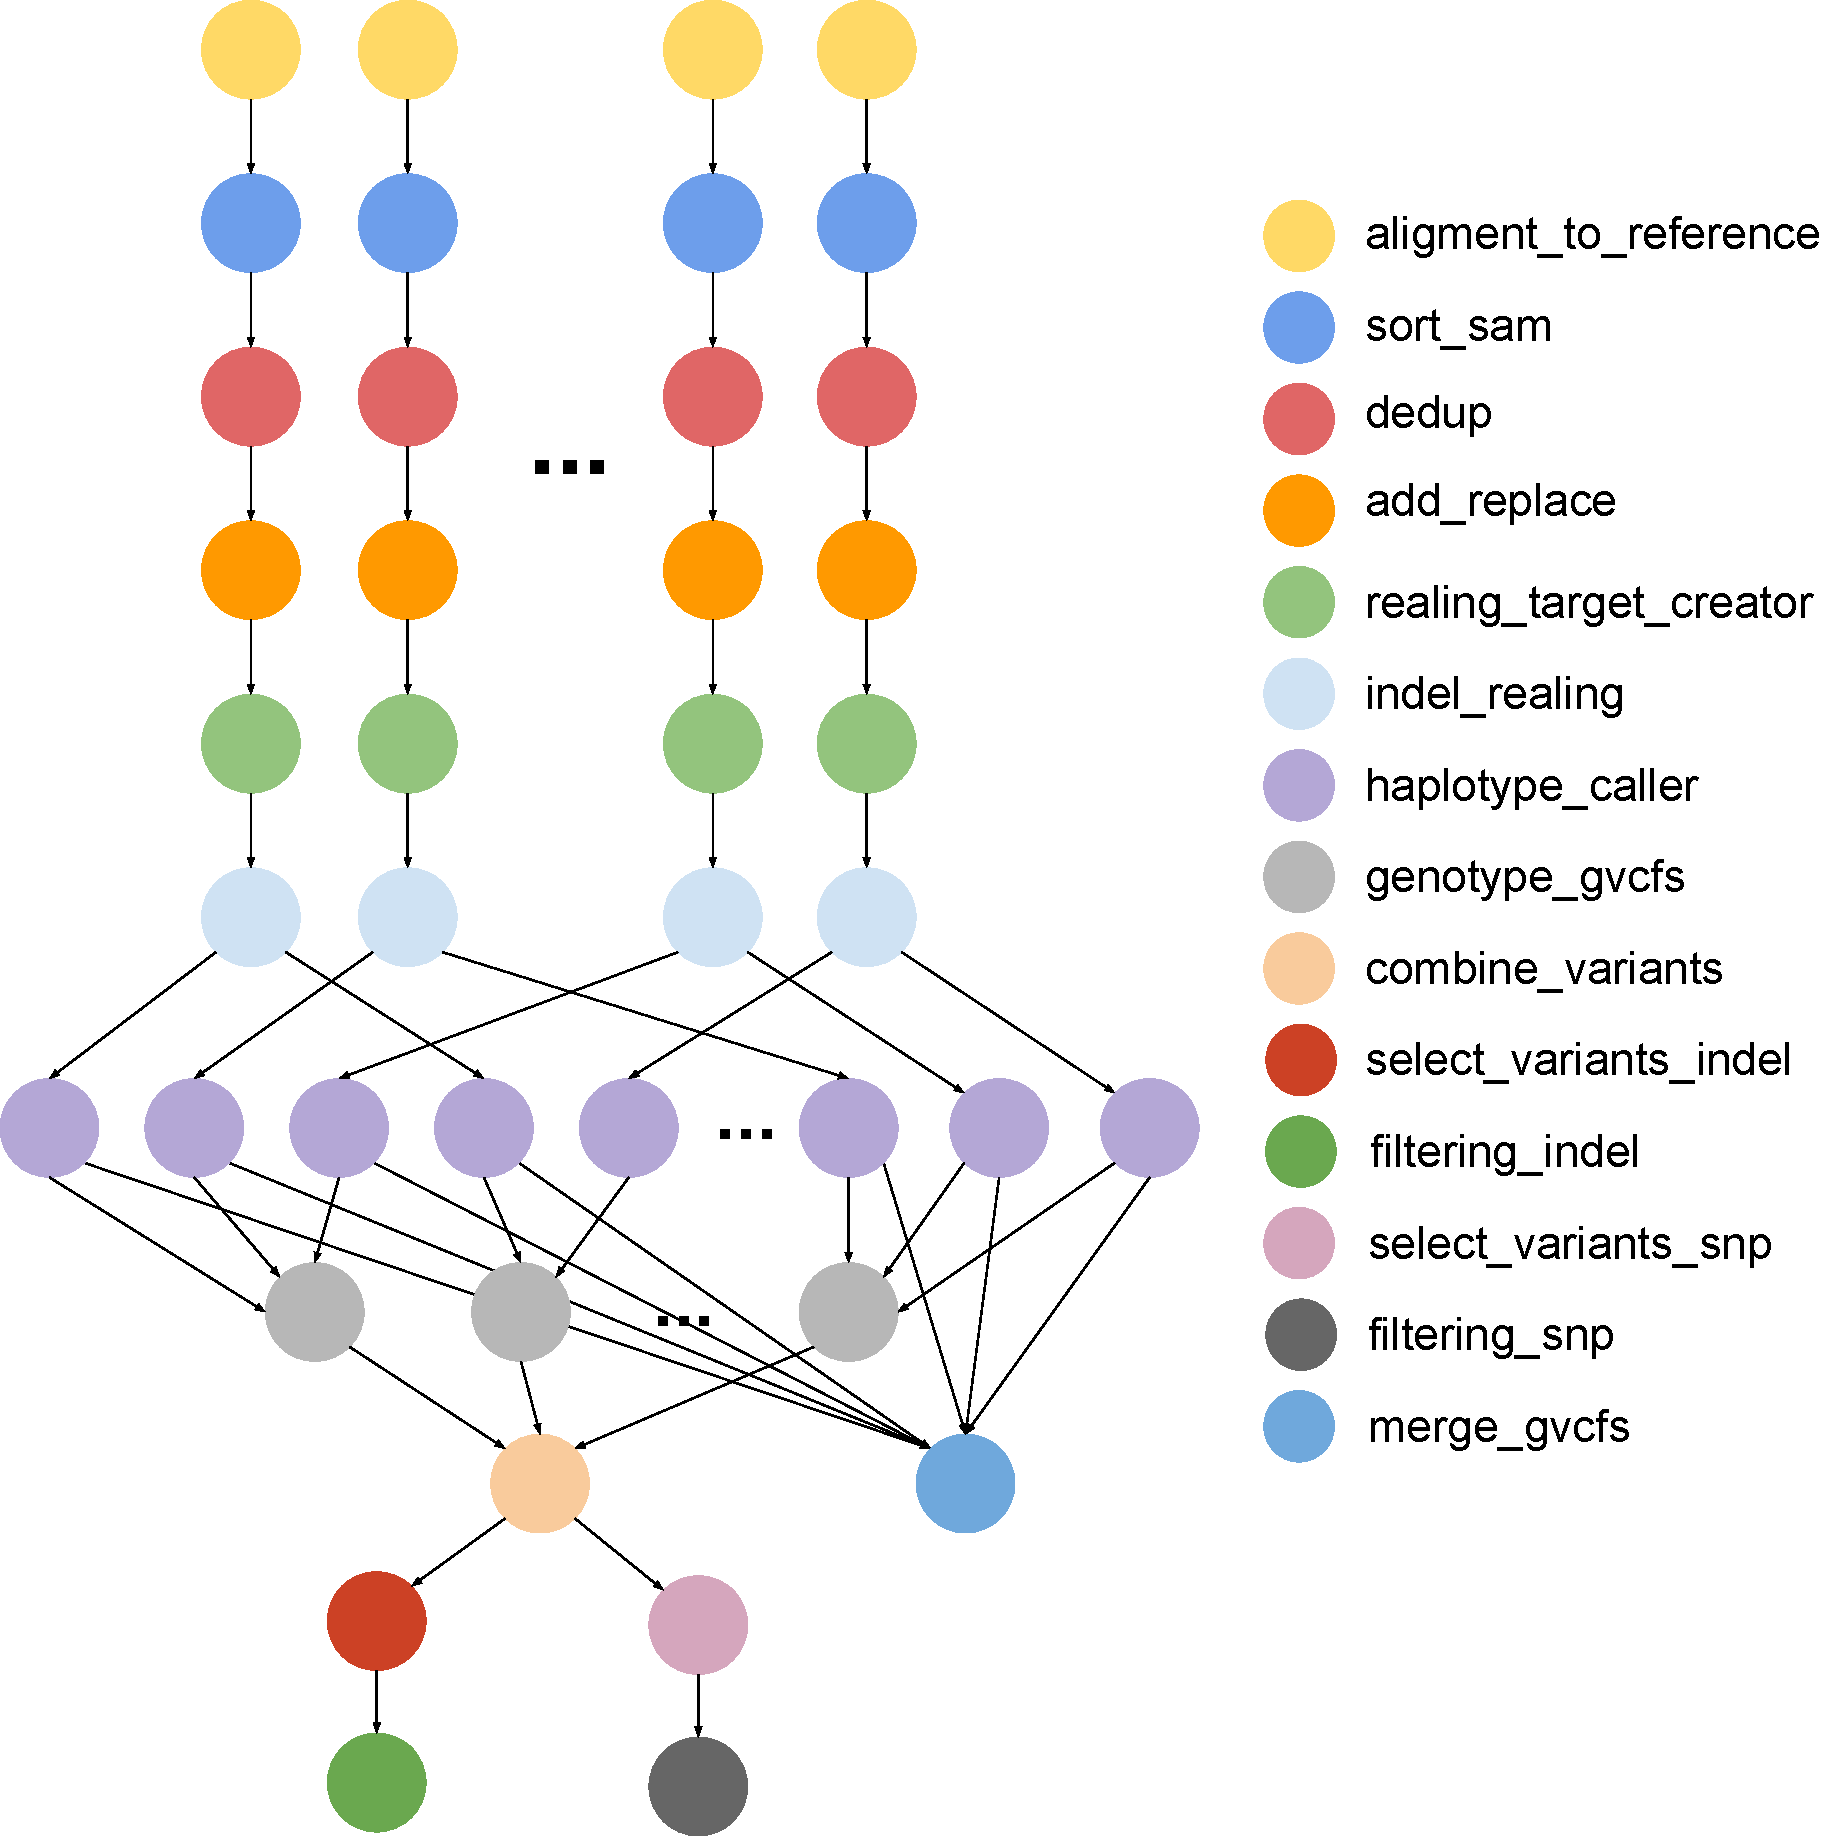
\includegraphics[width=0.95\linewidth]{figures/workflow-soybean}
	\caption{SoyKB workflow.}
	\label{fig:workflow-soykb}
\end{figure}



%%%
\subsection{Generating Semantic Annotations}

In this subsection, we present the annotations generated for each of the aforementioned
workflows and the Pegasus WMS using the WICUS ontology network.

\note{Restructure this section.}

As shown in Figure~\ref{fig:wicusflow}, the first step in the process of documenting a workflow is the annotation of the workflow DAX file. We use the \texttt{Workflow} domain ontology to describe the Montage workflow as 1) an individual that represents the top level workflow, and 2) a set of individuals representing its sub-workflows, one for each transformation. We then generate the necessary requirements, one for the top level workflow, which specifies the WMS requirements, and one for each subworkflow for defining the software components required by each transformation. 

In this experiment, we address two types of components: the WMS and the application related components. Figure~\ref{fig:annotations} shows a simplified overview of the annotations generated using the WICUS ontology network for the WMS and the three workflows studied in this work.


\paragraph{\textbf{WMS}}

 The WMS components include the workflow engine, in our case the Pegasus WMS, and its dependencies. Pegasus uses HTCondor as task manager, and both depend on Java and \texttt{wget} for running. We use the \texttt{Software} domain ontology to describe these components as individuals, and to represent their dependencies. The 3 components also depend on the operating system, which in our case is CentOS.

To describe the deployment of the WMS components, we studied their installation processes according to their documentation. We then defined a set of installation bash scripts for each of them. These scripts are included on the deployment plans of the components along with their configuration information.  
 
\paragraph{\textbf{Montage}}
 
Application components are described in the the Montage workflow's Transformation Catalog, where the binary file, version, and destination path are defined. These components are also described as individuals using the \texttt{Software} domain ontology. We use this information to generate the configuration parameters of the deployment script, which in this case is the same for all components. 

The script downloads the binary files from an online repository and copies them to the specified destination path. This process identified 59 software components for the Montage workflow that are annotated and included in the Software Components Catalog.

Then, the Transformation Catalog Annotator module relates each transformation requirement, defined using the \texttt{Workflow} domain ontology, to the application component, and therefore to the deployment information.
In this experiment, we define 9 Montage components that are linked to the requirements, and another two sub-components that are defined as dependencies in the software catalog (\emph{mDiffFit} depends on the \emph{mDiff} and \emph{mFitPlane} components).



\begin{figure*}[!htb]
	\centering
	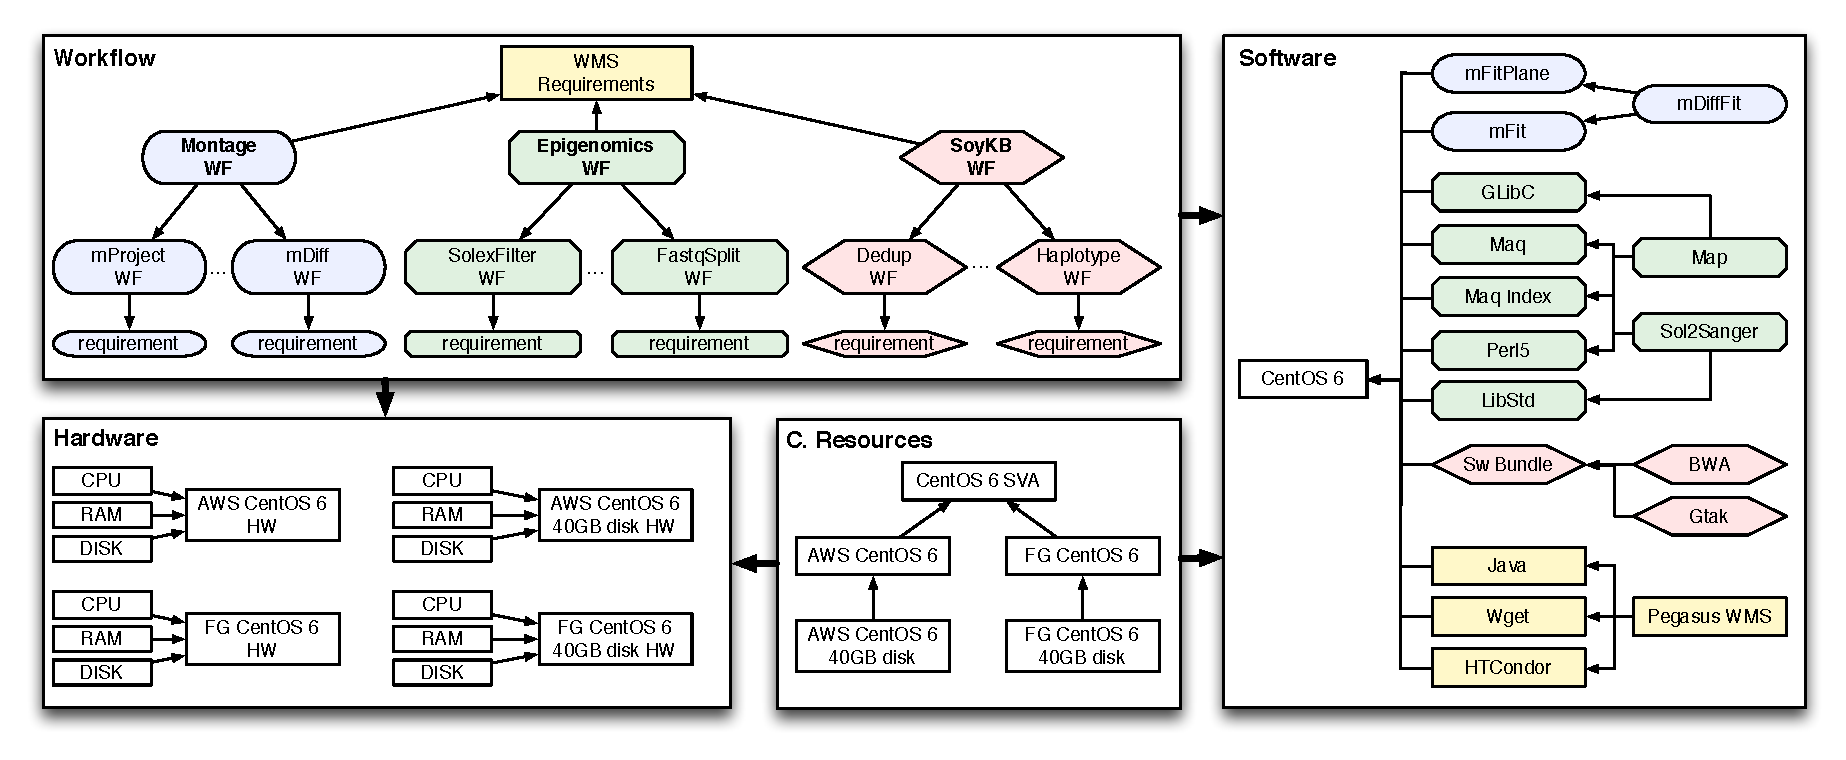
\includegraphics[width=\linewidth]{figures/annotations}
	\vspace{-20pt}
	\caption{Annotations for the Montage, Epigenomics, and SoyKB workflows using the WICUS ontology network (yellow rectangles represent the workflow component; blue squashed rectangles represent the Montage workflow; green bevelled rectangles represent the Epigenomics workflows; and red hexagons represent the SoyKB workflow).}
	\label{fig:annotations}
	\note{Rafael, missing dependency arrow between Gatk and SW bundle}

\end{figure*}

\note{Idafen, add decription of HW requirements of each workflow}


\paragraph{\textbf{Epigenomics}}

Following the same approach as in the previous case we have annotated the 8 components specified in the Epigenomics' Transformation Catalog. By analyzing the workflow dependencies we have also identified and annotated 6 software dependencies, which include software components and system libraries. 

These 8 main software components have been related to the 8 different types of steps depicted in figure \ref{fig:workflow-genome}.  Their dependencies include the Perl \cite{perl} interpreter, the GNU libc \footnote{http://www.gnu.org/software/libc/} and Libstdc++ \footnote{https://gcc.gnu.org/libstdc++/} libraries, and two other binaries from the Epigenomics  distribution, \emph{maq} and \emph{maqindex}.


\paragraph{\textbf{SoyKB}}

Even though SoyKB is the largest workflow in terms of its number of steps (around 670), of the three ones included in this work, it defines only four software components as dependencies. 

These components (\emph{bwa-wrapper}, \emph{bwa-wrapper},  \emph{gatk-wrapper}, and \emph{picard-wrapper}, \emph{software-wrapper},  \emph{gatk-wrapper}, \emph{picard-wrapper}) are software wrappers that call different libraries and binaries depending on the parameters used through the execution of the workflow. Those components are included on a software bundle that has to be deployed on the corresponding locations for the wrappers to be able to invoke it. Thus, a dependency for this bundle has been included in the Software Components Catalog.


\paragraph{\textbf{Computational resources}}

To describe computational resources we use the \texttt{Computing Resources} and \texttt{Hardware} domain ontologies. The Scientific Virtual Appliances Catalog includes the description of five virtual machine images, two for FutureGrid and other two for Amazon EC2. In both cases we generated conceptually equivalent machines, as they both provide CentOS 6 operating system, being the only difference their hardware configuration. 

Therefore, we generate five Image Appliances that are grouped into one single Scientific Virtual Appliance (CentOS 6 SVA). Depending on which providers are available, one or the other will be selected. Table \ref{tab:imgapps} summarizes the main characteristics of the five appliances we have annotated.


\begin{table}[h]
\begin{tabular}{l|lllll}
\multicolumn{1}{c|}{} 
Img. App. & AWS1 & AWS2 & FG1 & FG2 & Vagrant \\ \hline
RAM (GB) & 7 &  7 & 8 & 8 &  ?? \\ \hline
DISK (GB) &  40 &  5 &  40 & 5 & 50 \\ \hline
CPU freq (GHz) & 2.4  & 2.4 & 2.9 & 2.9  &  2.7 \\ \hline
CPU arch & \multicolumn{5}{c}{64 bits} \\ \hline
OS & \multicolumn{5}{c}{CentOS 6} \\ \hline
\end{tabular}
\caption{CentOS 6 Virtual Image Appliances}
\label{tab:imgapps}
\note{Idafen, improve the format of the table and complete vagrant info}
\end{table}

\paragraph{\textbf{Hardware requirements}}

For each of the workflows we have also analyzed which were hardware specifications required for executed them. Table \ref{tab:hwreqs} displays those requirements, describing the minimum threshold for each one of them. During the computational resource selection process we will consider that any machine with equal or higher hardware features than the ones specified will be a valid candidate for running the workflow. In cases such as the CPU frequency, in which we have not identified any specific capacity, we set this value to 0.



\begin{table}[h]
\begin{tabular}{l|llll}
\multicolumn{1}{c|}{} 
 & CPU (GHz) & CPU arch & RAM (GB) & DISK (GB) \\ \hline
Montage &  0 &  64 & 4 & 10 \\ \hline
Epigenomics &  0 &  64 &  4 & 4  \\ \hline
SoyKB & 0  & 64 & 4 & 4  \\ \hline
\end{tabular}
\caption{Workflow hardware requirements}
\label{tab:hwreqs}
\note{Idafen, improve the format of the table}
\end{table}

%%%
\subsection{Reproducing Workflow Executions.}

The last step on the process for achieving reproducibility in scientific workflows (Figure~\ref{fig:wicusflow}) is to execute the Infrastructure Specification Algorithm (ISA). The ISA combines the annotated data based on the 4 domain ontologies in order to find a suitable infrastructure specification that is able to run the workflow. The algorithm retrieves and propagates the WMS requirements of the top-level workflow (\texttt{Workflow} domain ontology) to its related sub-workflows. Requirements and software components are matched, and a dependency graph is built based on the relation between the requirements and the component dependencies. This graph is then used to compute the intersection between the set of software components from the SVA and the dependency graph of each sub-workflow. ISA selects the intersection where the value is maximized for each sub-workflow. Software components already available in the SVA are then removed from the chosen graph. To reduce the number of SVAs, the algorithm attempts to merge sub-workflows requirements into a single SVA. Requirements can be merged if all their software components are compatible. ISA also filters all those Image Appliances, belonging to the selected SVAs, that do not meet the hardware requirements specified for the workflow. Finally, ISA generates a script (either using PRECIP or Vagrant) with the set of required instructions to instantiate, configure, and deploy the computational resources and software components on the corresponding provider.

As introduced in~\cite{wicus} the ISA retrieves the corresponding information for the workflow and its dependencies from the annotations datasets. It calculates the dependencies and the compatibility between requirements and the available computational resources. It also takes into account the already installed software to avoid the unnecessary installation of components.

For this work we have added two main new features to the ISA. First of all we are now able to filter those Image Appliances that do not meet the hardware requirements specified for the target workflow (lines 25-27). Secondly have improved the script generation process, so we are now able to also generate Vagrant scripts. For this process we first generate an abstract deployment plan, defining the steps and scripts to be executed, along with their configuration parameters. The ISA then concretizes this plan into a PRECIP or Vagrant script depending on the resultant target provider (line 29).

A pseudo-code overview of the main steps of the ISA is listed in Listing \ref{lst:pseudo}.

\lstset{language=C++,
	  numbers=left,
	   numberstyle=\tiny\color{mygray},
           basicstyle=\ttfamily\scriptsize,
          breaklines=true,
          }
          
\begin{lstlisting}[caption={Pseudo-code overview of the ISA},label={lst:pseudo}]
WorkflowRequirementsDataset.load();

SVADataset.load();

SoftwareCatalogDataset.load();

Map<Workflow,List<Requirements>> wfSwReqs = 
  retrieveSwRequirements(WorkflowRequirementsDataset, WorkflowID);

Map<Workflow,List<Requirements>> propagatedWfSwReqs = 
  propagateSwReqs(wfSwReqs);

List<List<List<SWComponents>>> softwareComponents = getSoftwareComponents(propagatedWfSwReqs);

Map<Requirement,D-Graph<SWComponents>> softwareComponentsDependencyGraph = getSoftwareDependencies(softwareComponents);

List<SVA> availableSvas = getAvailableSvas(providersList);

Map<Requirements,SVA> maxCompatibilities = getCompatibilityIntersection(softwareComponentsDependencyGraph,availableSvas);

Map<Requirement,D-Graph<SWComponents>> substractedSwComponentsDepGraph = substractSoftwareComponents(softwareComponentsDependencyGraph, maxCompatibilities);

Map<SVA, List<Requirments>>mergedSvas= mergeSubworkflows(propagatedWfSwReqs, maxCompatibilities);

Map<Workflow,List<Requirements>> wfHwReqs =   retrieveHwRequirements(WorkflowRequirementsDataset, WorkflowID);

Map<SVA, List<Requirments>>filteredSvas= getCompatibleHwImageAppliances(mergedSvas,wfHwReqs);

generateScript(filteredSvas ,substractedSwComponentsDepGraph);

\end{lstlisting}


In this experiment, we execute ISA over the annotated data specifying the three different providers we work with. As result we obtain the abstract plans listed in listings \ref{lst:plan-montge}, \ref{lst:plan-epigenomics}, and \ref{lst:plan-soykb}. 


\begin{lstlisting}[caption={Abstract deployment plan of the Montage WF},label={lst:plan-montge}]
add...
\end{lstlisting}


\begin{lstlisting}[caption={Abstract deployment plan of the Epigenomics WF},label={lst:plan-epigenomics}]
add...
\end{lstlisting}


\begin{lstlisting}[caption={Abstract deployment plan of the SoyKB WF},label={lst:plan-soykb}]
  OPEN_SSH_CLIENTS_SOFT_STACK stack
   OPEN_SSH_CLIENTS_SOFT_COMP component
    OPEN_SSH_CLIENTS_DEP_STEP step
  OPEN_SSH_SERVER_SOFT_STACK stack
   OPEN_SSH_SERVER_SOFT_COMP component
    OPEN_SSH_SERVER_DEP_STEP step
  WGET_SOFT_STACK stack
   WGET_SOFT_COMP component
    WGET_DEP_STEP step
  CONDOR_CENTOS_6_5_SOFT_STACK stack
   CONDOR_CENTOS_6_5_SOFT_COMP component
    STOP_CONDOR_DEP_STEP step
    ADD_CONDOR_REPO_DEP_STEP step
    CONDOR_YUM_INSTALL_DEP_STEP step
    CLEAN_AND_SET_CONDOR_DEP_STEP step
    RESTART_DAEMONS_DEP_STEP step
  JAVA-1.7.0-OPENJDK.X86_64_SOFT_STACK stack
   JAVA-1.7.0-OPENJDK.X86_64_SOFT_COMP component
    JAVA-1.7.0-OPENJDK.X86_64_DEP_STEP step
  JAVA-1.7.0-OPENJDK-DEVEL.X86_64_SOFT_STACK stack
   JAVA-1.7.0-OPENJDK-DEVEL.X86_64_SOFT_COMP component
    JAVA-1.7.0-OPENJDK-DEVEL.X86_64_DEP_STEP step
  PEGASUS_WMS_CENTOS_6_5_SOFT_STACK stack
   PEGASUS_WMS_CENTOS_6_5_SOFT_COMP component
    ADD_PEGASUS_REPO_DEP_STEP step
    PEGASUS_YUM_INSTALL_DEP_STEP step
  SOFTWARE_TAR_GZ_SOFT_STACK stack
   SOFTWARE_TAR_GZ_SOFT_COMP component
    SOFTWARE_TAR_GZ_DEP_STEP step
  PICARD-WRAPPER_SOFT_STACK stack
   PICARD-WRAPPER_SOFT_COMP component
    PICARD-WRAPPER_DEP_STEP step
    PICARD-WRAPPER_2_DEP_STEP step
  SOFTWARE-WRAPPER_SOFT_STACK stack
   SOFTWARE-WRAPPER_SOFT_COMP component
    SOFTWARE-WRAPPER_DEP_STEP step
    SOFTWARE-WRAPPER_2_DEP_STEP step
  GATK-WRAPPER_SOFT_STACK stack
   GATK-WRAPPER_SOFT_COMP component
    GATK-WRAPPER_DEP_STEP step
    GATK-WRAPPER_2_DEP_STEP step
  BWA-WRAPPER_SOFT_STACK stack
   BWA-WRAPPER_SOFT_COMP component
    BWA-WRAPPER_DEP_STEP step
    BWA-WRAPPER_2_DEP_STEP step
\end{lstlisting}

In all cases, the algorithm is able to concretize the abstract plan either to a PRECIP or a Vagrant script (depending on the specified provider). Each generated script is composed by the following main sections:

\begin{itemize}

	\item \emph{Experiment Creation}: generates a new experiment using the given VM image ID and the user credentials for the selected infrastructure provider;
    	    
	\item \emph{Software Deployment}: executes the set of instructions defined on the deployment plan of each software component to install and configure the required software to execute the workflow. In this section, both the workflow management system and the application are deployed with their dependencies;

	\item \emph{User Setup}: creates a user account on the VM (if it does not exist) and configures the necessary SSH keys to enable file transfers and execution. This account will be used to run the workflow;
	   
	\item \emph{Data Stage and Workflow Execution}: stages all the input data of the Montage workflow on the VM, and launches the workflow execution. Since our work is focused on infrastructure reproducibility, data and workflow management are not covered in our approach.

\end{itemize}

\noindent Note that all the configuration and deployment commands (first 3 sections) require superuser privileges on the VM. The workflow execution, however, is performed under the user account created in the third section.


\note{Idafen, modify this including the results of the 3 WFs, and how we check results are correct}.

We executed the scripts on their corresponding platforms. Both executions succeeded on deploying and running the Montage workflow, the Pegasus WMS, and their dependencies. We also performed the same execution of the Montage workflow in a predefined VM image, where the execution environment is already in place. Results show that the VM execution environments deployed by both scripts are equivalent to the former one. In addition, we used a perceptual hash tool\footnote{pHash - \url{http://www.phash.org}} to compare the resulting image (0.1 degree image of the sky) generated by both executions against the one generated by the baseline execution. We obtained a similarity factor of 1.0 (over 1.0) with a threshold of 0.85, which means the images are identical. Therefore we are obtaining the same results as the original workflow. In this work we do not aim to reproduce either the performance or the execution time of the original experiment.



All the original and generated scripts are available as part of the experimental material included in the Research Object (RO)~\cite{researchObjects} associated with this paper\footnote{\url{http://pegasus.isi.edu/publications/FGCS(CREATE-RO!)}}. This RO also contains pointers to the software and resources used in this experiment.